% RMS vs EDF comparison — tau1(C=2,T=4) tau2(C=3,T=6), U=1.0
% Top panel: RMS (tau1>tau2) — tau2 misses deadline at t=6
% Bottom panel: EDF — all deadlines met
\documentclass[border=5pt]{standalone}
\usepackage{lmodern}
\usepackage{tikz}
\usetikzlibrary{arrows.meta}

\definecolor{kmblue}{HTML}{003874}
\definecolor{kmgold}{HTML}{BA9224}
\definecolor{rtgreen}{HTML}{1F9D55}
\definecolor{rtred}{HTML}{E3342F}
\definecolor{axgray}{HTML}{888888}
\definecolor{dkgray}{HTML}{555555}

\begin{document}
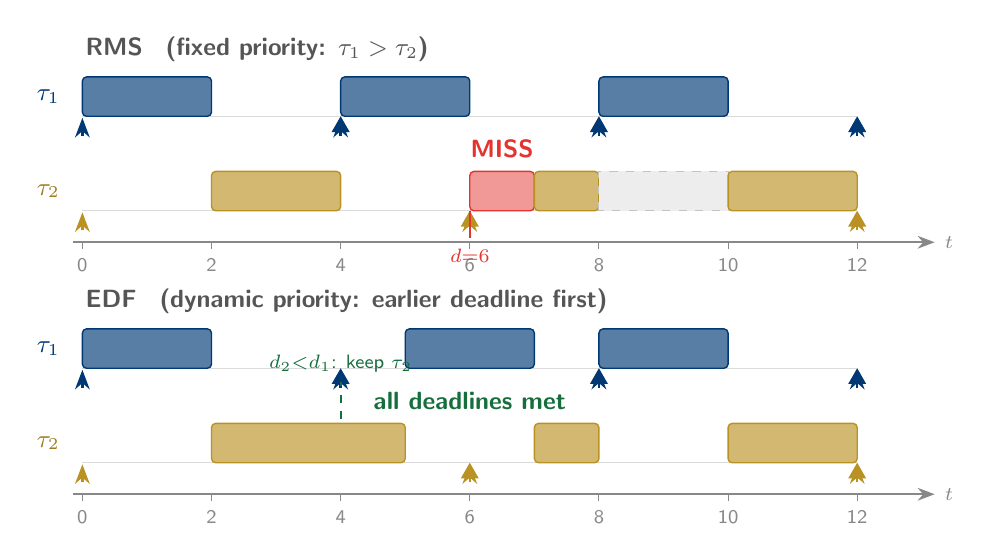
\begin{tikzpicture}[>=Stealth,font=\sffamily,x=0.82cm,y=1cm]

  \def\h{0.50}

  % =====================================================================
  % TOP PANEL — RMS (fixed priority: tau1 > tau2)
  % Schedule [0,12]:
  %   tau1: [0,2] [4,6] [8,10]
  %   tau2: [2,4] [6,7](MISS) [7,8] preempted [10,12]
  % =====================================================================
  \def\yA{5.4}  % tau1 (RMS) row base
  \def\yB{4.2}  % tau2 (RMS) row base
  \def\Yoff{4.0} % vertical offset between panels

  % panel label
  \node[dkgray,font=\sffamily\small\bfseries,anchor=west] at (-0.1,6.25)
        {RMS \enspace (\emph{fixed priority:} $\tau_1 > \tau_2$)};

  % time axis
  \draw[axgray,line width=0.7pt,->] (-0.15,3.8) -- (13.2,3.8)
        node[right,font=\sffamily\scriptsize] {$t$};
  \foreach \t in {0,2,4,6,8,10,12} {
    \draw[axgray] (\t,3.8) -- (\t,3.72)
          node[below,font=\sffamily\scriptsize,axgray] {\t};
  }

  % row guides
  \draw[axgray!30,line width=0.4pt] (0,\yA) -- (12,\yA);
  \draw[axgray!30,line width=0.4pt] (0,\yB) -- (12,\yB);

  % task labels
  \node[anchor=east,kmblue,font=\sffamily\small\bfseries]
        at (-0.2,\yA+0.5*\h) {$\tau_1$};
  \node[anchor=east,kmgold!85!black,font=\sffamily\small\bfseries]
        at (-0.2,\yB+0.5*\h) {$\tau_2$};

  % tau1 (RMS): [0,2] [4,6] [8,10]
  \foreach \s/\e in {0/2, 4/6, 8/10} {
    \fill[kmblue!65,rounded corners=1.5pt]
          (\s,\yA) rectangle (\e,\yA+\h);
    \draw[kmblue,line width=0.5pt,rounded corners=1.5pt]
          (\s,\yA) rectangle (\e,\yA+\h);
  }

  % tau2 (RMS): [2,4] normal, then [6,7] MISS, [7,8] then preempted, [10,12]
  \fill[kmgold!65,rounded corners=1.5pt]
        (2,\yB) rectangle (4,\yB+\h);
  \draw[kmgold,line width=0.5pt,rounded corners=1.5pt]
        (2,\yB) rectangle (4,\yB+\h);
  % [6,7] — runs late, missed deadline at t=6
  \fill[rtred!50,rounded corners=1.5pt]
        (6,\yB) rectangle (7,\yB+\h);
  \draw[rtred,line width=0.5pt,rounded corners=1.5pt]
        (6,\yB) rectangle (7,\yB+\h);
  % [7,8] job2 starts, [8,10] preempted gap
  \fill[kmgold!65,rounded corners=1.5pt]
        (7,\yB) rectangle (8,\yB+\h);
  \draw[kmgold,line width=0.5pt,rounded corners=1.5pt]
        (7,\yB) rectangle (8,\yB+\h);
  \fill[axgray!15] (8,\yB) rectangle (10,\yB+\h);
  \draw[axgray!50,line width=0.4pt,dashed] (8,\yB) rectangle (10,\yB+\h);
  \fill[kmgold!65,rounded corners=1.5pt]
        (10,\yB) rectangle (12,\yB+\h);
  \draw[kmgold,line width=0.5pt,rounded corners=1.5pt]
        (10,\yB) rectangle (12,\yB+\h);

  % release arrows (RMS)
  \foreach \t in {0,4,8,12}
    \draw[kmblue,line width=0.9pt,->] (\t,\yA-0.25) -- (\t,\yA-0.02);
  \foreach \t in {0,6,12}
    \draw[kmgold,line width=0.9pt,->] (\t,\yB-0.25) -- (\t,\yB-0.02);

  % deadline marks (RMS)
  \foreach \t in {4,8,12}
    \fill[kmblue] (\t,\yA) -- (\t-0.14,\yA-0.20) -- (\t+0.14,\yA-0.20) -- cycle;
  \foreach \t in {6,12}
    \fill[kmgold] (\t,\yB) -- (\t-0.14,\yB-0.20) -- (\t+0.14,\yB-0.20) -- cycle;

  % MISS annotation
  \node[rtred,font=\sffamily\bfseries\small] at (6.5,\yB+\h+0.28) {MISS};
  \draw[rtred,line width=0.8pt] (6,\yB) -- (6,\yB-0.35)
        node[below,font=\sffamily\scriptsize] {$d{=}6$};

  % =====================================================================
  % BOTTOM PANEL — EDF (dynamic priority: always run earliest deadline)
  % Schedule [0,12]:
  %   tau1: [0,2] [5,7] [8,10]
  %   tau2: [2,5] [7,8] [10,12]
  % =====================================================================
  \def\yC{2.2}  % tau1 (EDF) row base
  \def\yD{1.0}  % tau2 (EDF) row base

  % panel label
  \node[dkgray,font=\sffamily\small\bfseries,anchor=west] at (-0.1,3.05)
        {EDF \enspace (\emph{dynamic priority:} earlier deadline first)};

  % time axis
  \draw[axgray,line width=0.7pt,->] (-0.15,0.6) -- (13.2,0.6)
        node[right,font=\sffamily\scriptsize] {$t$};
  \foreach \t in {0,2,4,6,8,10,12} {
    \draw[axgray] (\t,0.6) -- (\t,0.52)
          node[below,font=\sffamily\scriptsize,axgray] {\t};
  }

  % row guides
  \draw[axgray!30,line width=0.4pt] (0,\yC) -- (12,\yC);
  \draw[axgray!30,line width=0.4pt] (0,\yD) -- (12,\yD);

  % task labels
  \node[anchor=east,kmblue,font=\sffamily\small\bfseries]
        at (-0.2,\yC+0.5*\h) {$\tau_1$};
  \node[anchor=east,kmgold!85!black,font=\sffamily\small\bfseries]
        at (-0.2,\yD+0.5*\h) {$\tau_2$};

  % tau1 (EDF): [0,2] [5,7] [8,10]
  \foreach \s/\e in {0/2, 5/7, 8/10} {
    \fill[kmblue!65,rounded corners=1.5pt]
          (\s,\yC) rectangle (\e,\yC+\h);
    \draw[kmblue,line width=0.5pt,rounded corners=1.5pt]
          (\s,\yC) rectangle (\e,\yC+\h);
  }

  % tau2 (EDF): [2,5] [7,8] [10,12]
  \foreach \s/\e in {2/5, 7/8, 10/12} {
    \fill[kmgold!65,rounded corners=1.5pt]
          (\s,\yD) rectangle (\e,\yD+\h);
    \draw[kmgold,line width=0.5pt,rounded corners=1.5pt]
          (\s,\yD) rectangle (\e,\yD+\h);
  }

  % release arrows (EDF)
  \foreach \t in {0,4,8,12}
    \draw[kmblue,line width=0.9pt,->] (\t,\yC-0.25) -- (\t,\yC-0.02);
  \foreach \t in {0,6,12}
    \draw[kmgold,line width=0.9pt,->] (\t,\yD-0.25) -- (\t,\yD-0.02);

  % deadline marks (EDF)
  \foreach \t in {4,8,12}
    \fill[kmblue] (\t,\yC) -- (\t-0.14,\yC-0.20) -- (\t+0.14,\yC-0.20) -- cycle;
  \foreach \t in {6,12}
    \fill[kmgold] (\t,\yD) -- (\t-0.14,\yD-0.20) -- (\t+0.14,\yD-0.20) -- cycle;

  % all-met annotation
  \node[rtgreen!70!black,font=\sffamily\bfseries\small]
        at (6,\yD+\h+0.28) {all deadlines met};

  % EDF priority switch annotation at t=4
  \draw[rtgreen!70!black,line width=0.7pt,dashed]
        (4,\yD+\h+0.05) -- (4,\yD+\h+0.52);
  \node[rtgreen!70!black,font=\sffamily\scriptsize,above]
        at (4,\yD+\h+0.52) {$d_2{<}d_1$: keep $\tau_2$};

\end{tikzpicture}
\end{document}
